% Chapter Template

\part {Search for heavy neutral leptons}


\chapter{Heavy Neutral Leptons} 
\label{Chapter3} 


In the Standard Model, all the fermions are known to have both, left and right handed chirality, the only exception comes from the neutrinos.

The recent neutrino oscillation experiments have clearly and definitely shown that neutrinos are massive; thus in this scenario, including the hypothesis of the existence of the right handed neutrinos, $\nu_{R}$ or \emph{Heavy Neutral Leptons} (HNLs), the light $\nu_{SM}$ flavor oscillations can be explained via the type I seesaw mechanism~\cite{MINKOWSKI1977421}~\cite{gellmann2013complex}~\cite{PhysRevLett.44.912}~\cite{PhysRevD.22.2227}.
Other consideration comes from the possibility to consider the $\nu_{R}$ as part of the explanations for the baryon asymmetry of the universe; the mixing between $\nu_{R}$ violates \emph{CP} and the interaction of the $\nu_{R}$ may potentially generate a matter-antimatter asymmetry in the early stage of the formation of the universe~\cite{Canetti_2012}~\cite{KUZMIN198536}.

These few examples, which are going to be explored later on, show already the relevance and the interest of the HNL program and the strong motivations behind the existence of the $\nu_{R}$.

\section{Neutrino Portal} \label{sec:neutrinoPortal}
The \emph{neutrino portal} is determined as coupling of one or more dark fermions $N$ ($N_{I} = 1,2,...$ $\mathcal{N}$), sterile with respect to the SM gauge interactions to the gauge-invariant operator ($\bar{L}_{\alpha}  \cdot \widetilde \Phi$); the general form of the neutrino portal could be displayed as: 
\begin{equation}
\label{eq:neutrinoportal}
\mathcal{L}_{vector} = \mathcal{L}_{SM} + \mathcal{L}_{DS} + \sum F_{\alpha I} (\bar{L}_{\alpha}  \cdot \widetilde \Phi)N_{I} + h.c.
\end{equation}

where the summation loops over the flavor of lepton doublets ${L}_{\alpha}$ ( $\alpha = e,\; \mu, \: \tau$) and the number of available HNLs $N_{I}$; $F_{\alpha I} $ are the Yukawa couplings and $\Phi$ is the Higgs doublet. The term $\mathcal{L}_{DS}$ should contain the mass term of HNL which can be both Majorana or Dirac~\cite{Alekhin_2016}.
Fixing the $\Phi$ to its vacuum expectation value, $\widetilde \Phi = \frac{1}{\sqrt{2}} \binom{v}{0}$, and diagonalize the mass term of the dark fermions, the term~\ref{eq:neutrinoportal} brings to the quadratic mixing of the neutrinos $\nu_{\alpha}$ with the $N_{I}$; this mixing is parametrized by a matrix $V.$ In the minimal HNL models, the elements of the matrix $V$ control both the production and the decay of the HNLs (see fig.~\ref{fig:c3diagram_decay}). 
If $\mathcal{N} = 3$, there is a right-chiral counterpart for each $\nu_{SM}$, see fig.~\ref{fig:c3sm_extension}. The fermion $N_I$ can have mass $M_I$ which is independent  of the value of $F_{\alpha I}$.
\begin{figure}[t!]
  \centering
  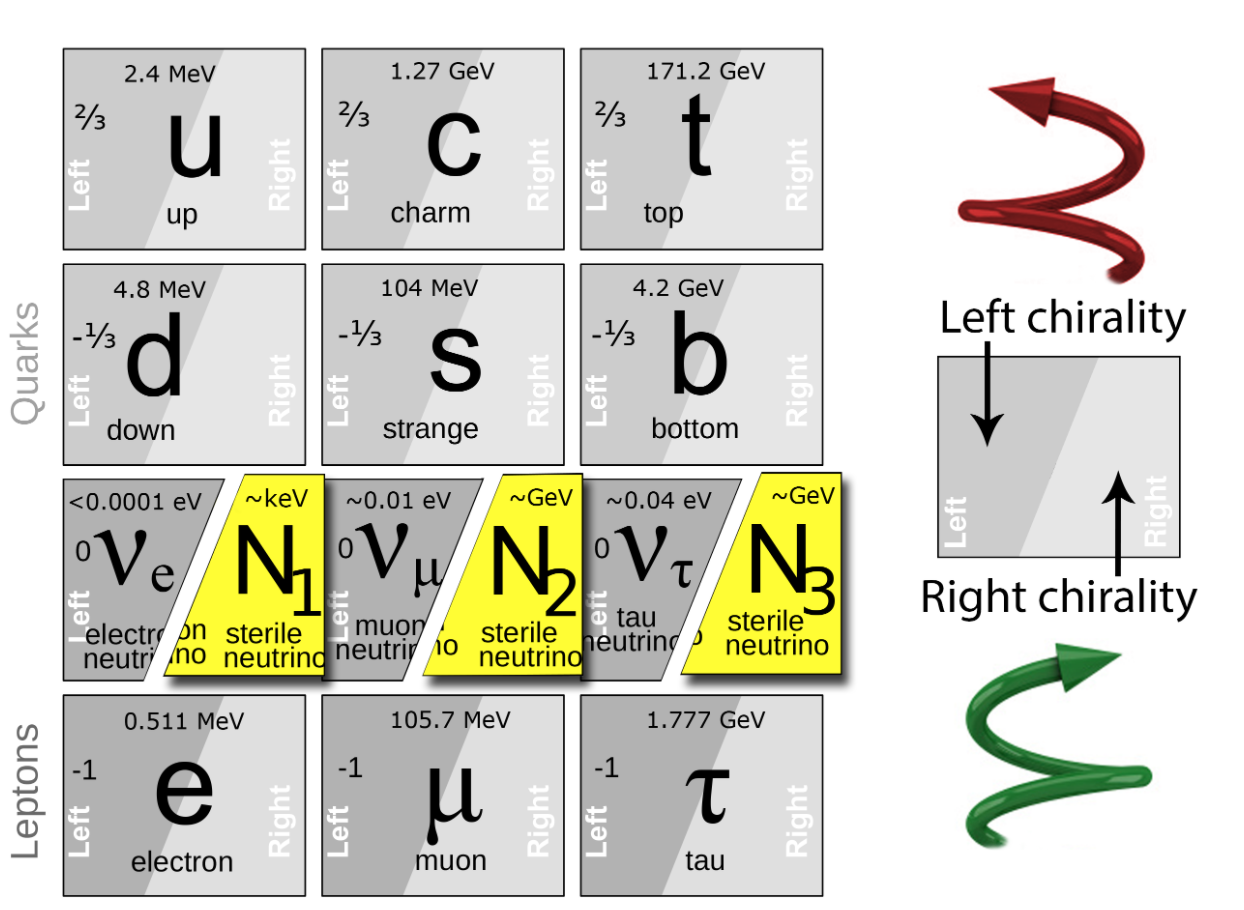
\includegraphics[width=.60\textwidth]{Figures/c3/SM_extension}
    \caption{There are 3 SM neutrinos $\nu_{e}, \; \nu_{\mu}, \;\nu_{\tau}$ which are massless and always left-chiral; 3 right-chiral counterparts are added $N_{1}, \; N_{2}, \;N_{3}$. They are sterile so they do not feel the electric, weak and strong forces}
  \label{fig:c3sm_extension}
\end{figure}

Considering the existing searches and considering a model-indipendent phenomenological approach, we could assume the existence of only a \emph{single} sufficiently light HNL can be kinematically accessible at the accelerator experiments; see full overview in~\cite{Atre_2009}. There are then only two free parameters to be constrained: the mass $M_I$ of the HNL and its coupling with an SM neutrino of flavor $\alpha$ controlled by the Yukawa coupling $F_{\alpha I}$. Without any signal excess, upper limits are settled on the mixing parameter $|V^2_{\alpha I}|$ ($= |F^2_{\alpha I}|$) as function of the $M_I$ for a given flavor $\alpha$. It is very often assumed that in the matrix $V$ the other mixing elements for different flavors are zero; this latter consideration, in spite of the fact that does not translate into a valid concrete model, it is very useful to extract generic limits on the single $|V^2_{\alpha I}|$ without involving any model dependent hierarchy between the different flavor mixings. 
\begin{figure}[t!]
  \centering
  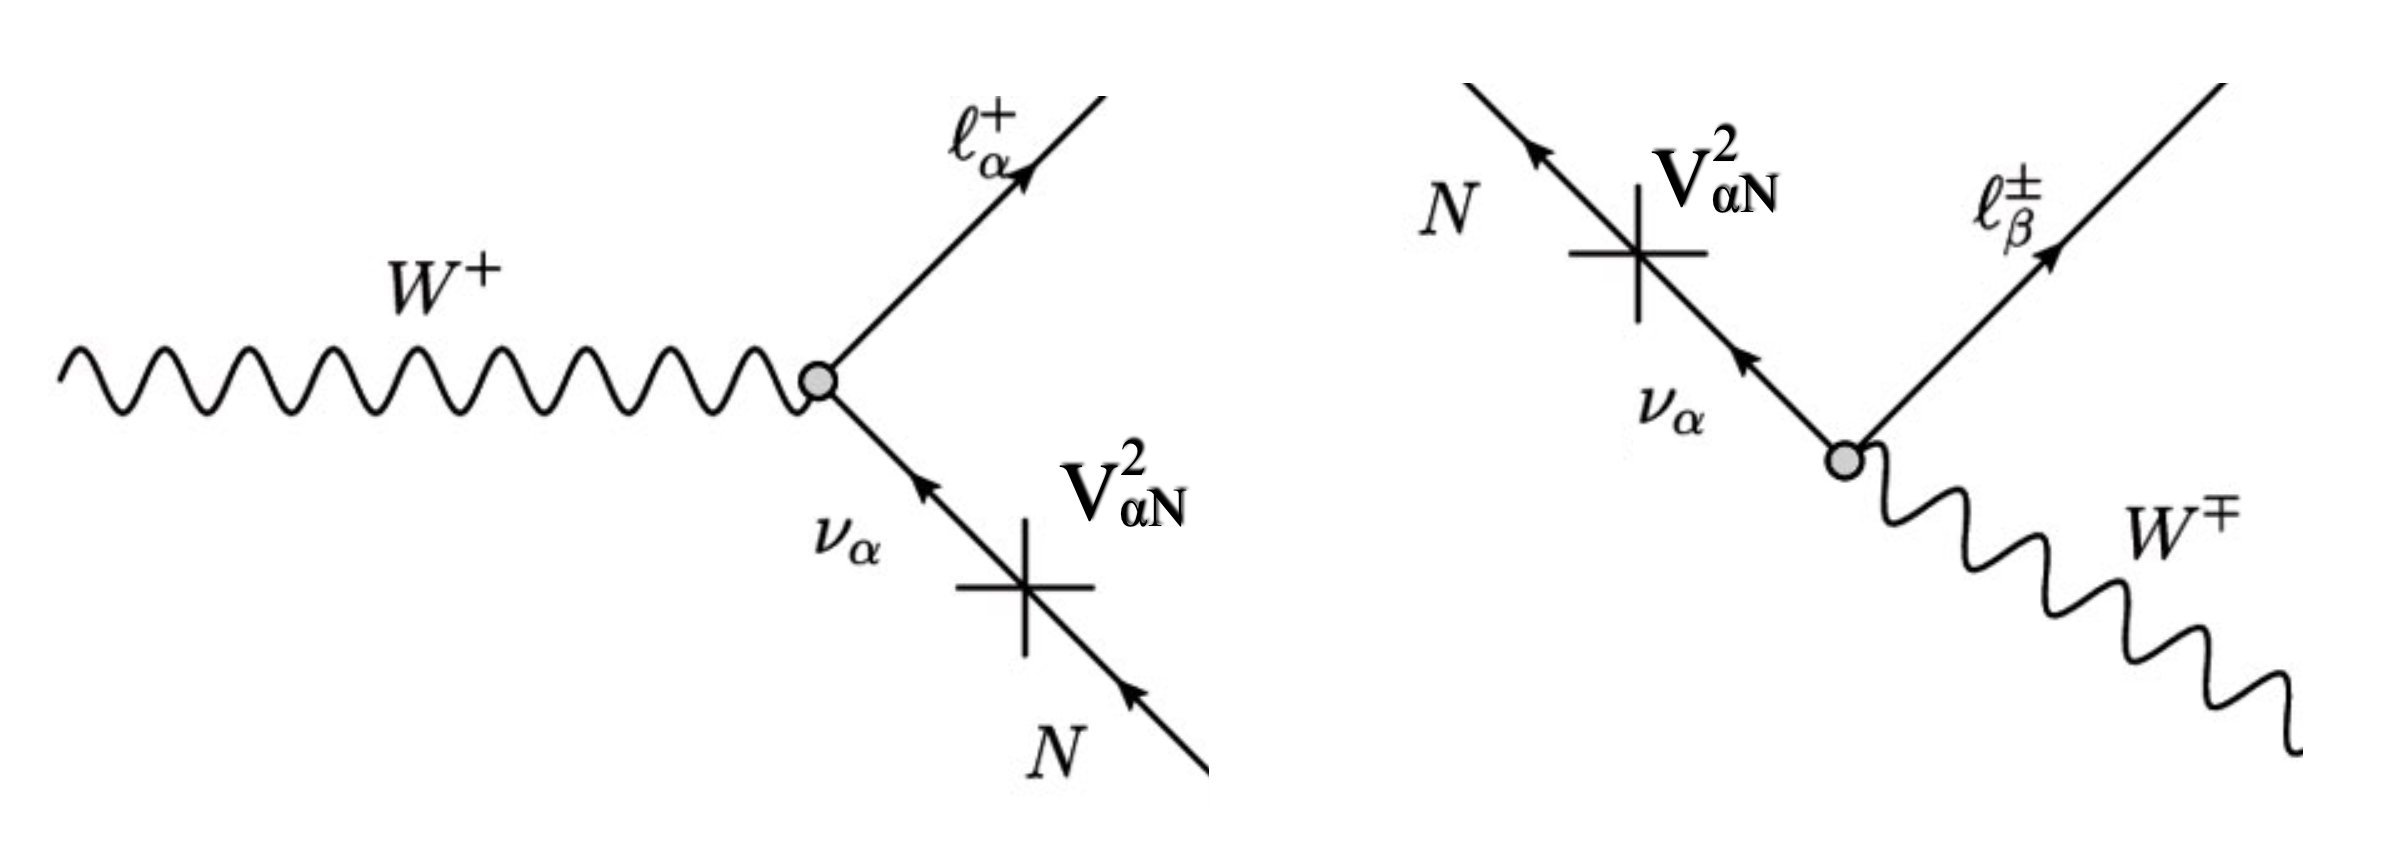
\includegraphics[width=.80\textwidth]{Figures/c3/diagram_decay}
    \caption{Production (left) and decay (right) of the particle $N_{I}$.}
  \label{fig:c3diagram_decay}
\end{figure}

\section{Heavy neutral lepton formalism and extension of the standard model}
To set up our notation and convention, we first discuss the formalism for the simplest
extension of the SM which includes right handed singlets. Also in this section, we present
the current constraints on the mass and mixing of a heavy neutrino from various direct
detection experiments, accelerator searches and electroweak precision constraints.
\subsection{Seesaw formula}\label{sec:seesaw}
The most general renormalisable Lagrangian for the neutrino masses includes both the Dirac and Majorana mass terms. The SM Lagrangian $\mathcal{L}_{SM}$ is extended adding $\mathcal{N}$ right-handed neutrinos $N_I$: (for notations see Eq.~\ref{eq:neutrinoportal}).
\begin{equation}
\label{eq:fullSMLag}
 \mathcal{L} = \mathcal{L}_{SM}+ i \bar N_I \partial_\mu \gamma^\mu N_I -
  \left(F_{\alpha I} \,\bar L_\alpha N_I \tilde \phi 
    - \frac{M_I}{2} \; \bar {N_I^c} N_I + h.c.\right)
\end{equation}
As already explained in the previous section (~\ref{sec:neutrinoPortal}), these $N_I$ are neutral with respect to all the gauge interactions of the SM, thus are called \emph{sterile neutrinos} or \emph{gauge-singlet fermions}.
In the Higgs phase, the term~\ref{eq:neutrinoportal} brings to the $\nu_{\alpha} - N_I$ mixing. As result the \emph{charge eigentatses} of the $\mathcal{L}_{SM}$ (~\ref{eq:fullSMLag}) do not coincide with the \emph{mass eigenstates}, which can be extracted diagonalizing the following matrix:
\begin{equation}
\label{eq:matrixmass}
 \mathcal{M}_{\nu,N} = 
\begin{pmatrix}
0 & m_D\\
m^{T}_{D} & M_I
\end{pmatrix}
\end{equation}
with $m_D = 3 \times  \mathcal{N}$ Dirac mass matrix, $(m_D)_{\alpha I} = F_{\alpha I}v, \; v = \sqrt{2}\langle \Phi \rangle$ and $M_I$ is $\mathcal{N} \times \mathcal{N}$ matrix of Majorana masses.

Considering the relation between $M_I$ and $m_D$, we could explore two interesting extreme limits:
\paragraph {Pure Majorana neutrino, $m_D \ll M_I$.}
In this limit, the mass matrix give rise to 3 almost pure right-handed neutrinos with heavy Majorana mass $M_I$ and 3 almost pure left-handed neutrinos with light Majorna mass $m_\nu = - (vm_D)^{T}M^{-1}_{I}(vm_D)$ which are the 3 eigenvalues of the matrix $(\mathcal{M}_{\nu})_{\alpha \beta}$. This mechanism is then referred to as the \emph{seesaw mechanism}\footnote{This mechanism is usually called \emph{Type-I seesaw}. \emph{Type-II seesaw} has an extra SU(2) triplet scalar~\cite{Deppisch_2015}; in \emph{Type-III seesaw} an extra fermion in the adjoint of SU(2) is added to the model~\cite{Foot:1988aq}}~\cite{MINKOWSKI1977421}~\cite{Mohapatra:1979ia}~\cite{Yanagida:1979as}.
\begin{figure}[t!]
  \centering
  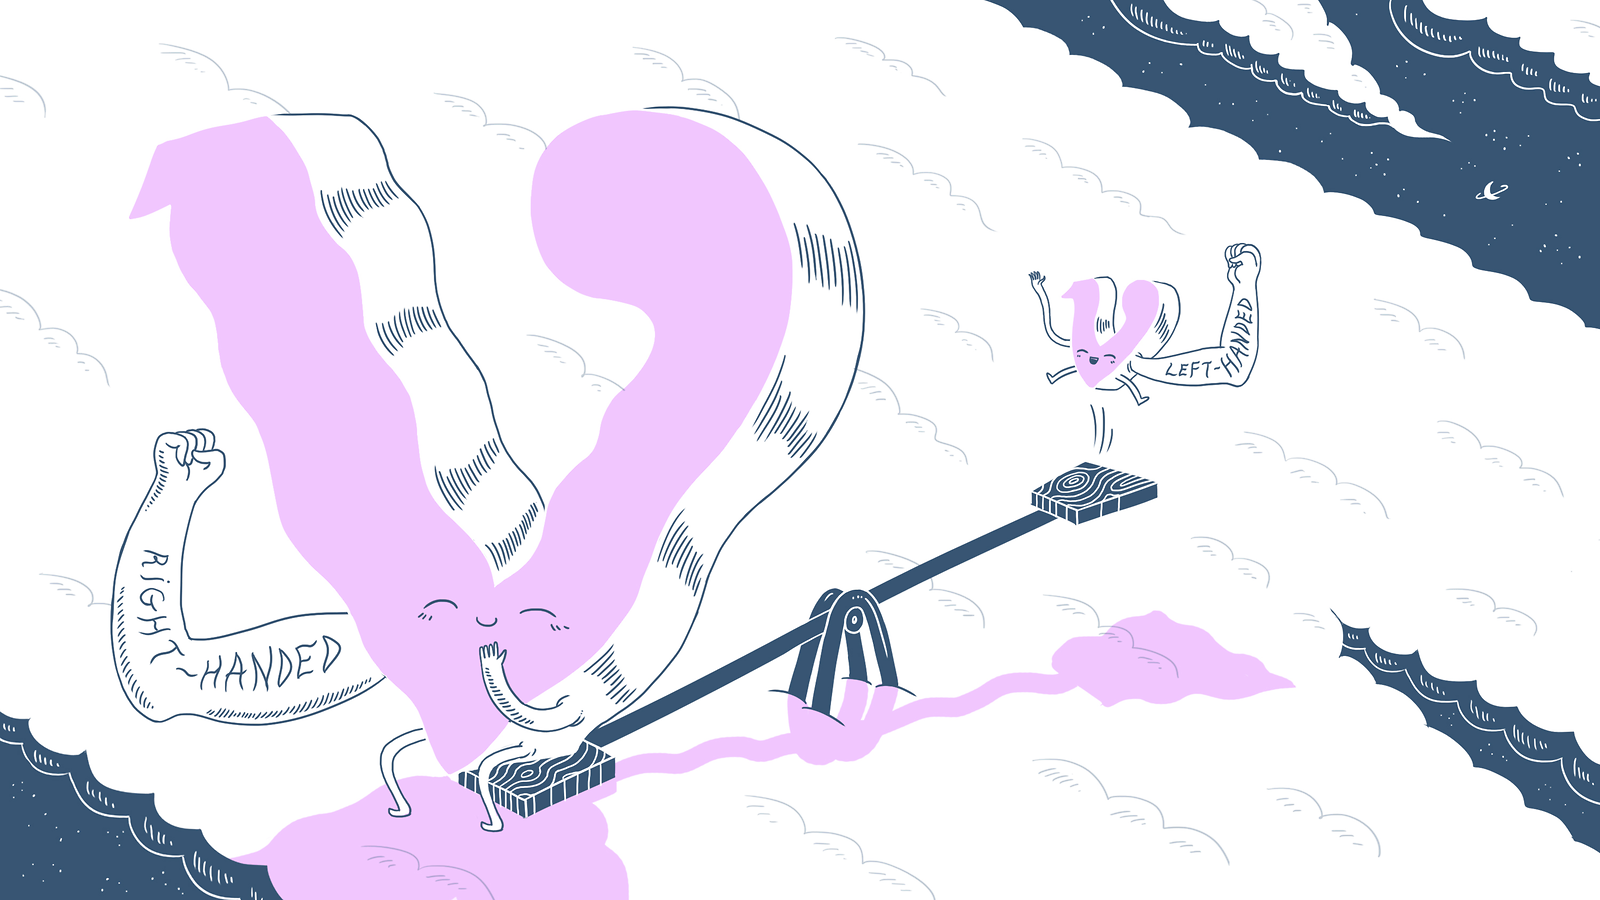
\includegraphics[width=.60\textwidth]{Figures/c3/funny.png}
    \caption{Silly representation of the \emph{seesaw mechanism}~\cite{funny}. Note that for a fix value of $m_D$, higher is value of the $m^{R}_I$ lower is the one of the $m^{L}_I$ and vice-versa, from this the \emph{seesaw} name.}
  \label{fig:c3funny}
\end{figure}
There are then the other $\mathcal{N}$ eigenstates of the $\mathcal{M}_{\nu,N}$ which almost coincide with the $N_I$ up to a small admixture of $\nu_\alpha$.
The magnitude of this mixing is given by the ration of the Dirac and Majorana masses $\rightarrow$ \emph{mixing angle} or \emph{active-sterile mixing}:

\begin{equation}
 V^2_{\alpha I} \equiv \frac{v^{2}|F_{\alpha I}|^2}{M^{2}_{I}} \ll 1
\end{equation}
It generates the 9 measurable neutrino mass parameters from $m_D$ and $M_I$, that contain 18 unknown parameters to the Lagrangian: $number\; of \; HNL \; parameters = 7 \times \mathcal{N} - 3$. $\mathcal{N}$ are the real Majorana masses $M_I$ plus $3\times \mathcal{N}$ complex Yukawa coupling $F_{\alpha I}$ minus 3 phases which go to the redefinitions of $\nu_e, \; \nu_\mu,\; \nu_\tau$.

\paragraph {Pure Dirac neutrino, $M_I \ll m_D$.}
In this limit, the mass matrix give rise to 3 Dirac neutrinos $\Psi = (\nu_L,\:\bar{\nu_R})$ with mass $m_\nu = m_D$. To obtain the observed neutrino masses then the coupling $F_{\alpha I} \sim 10^{-12}$ which is much smaller than the SM Yukawa couplings.

\vspace{5mm} 
This paragraph below is freely inspired by the overview given by R.D. Kauber here~\cite{webpage_seesaw}.
\subsubsection{Considerations on Majorana and Dirac neutrinos}
\paragraph {Distinction between Majorana and Dirac terms.}
The nomenclature "Majorana" is used to define different things and it is important for the following chapters to clarify the meaning. In the Sec.~\ref{sec:seesaw} \emph{Majorana} and \emph{Dirac} are used to refer to the mass terms in the Lagrangian~\ref{eq:fullSMLag}. The additional meaning is related to the type of neutrino. A \emph{Majorana} particle is defined as a particle that is its own antiparticle.  A Dirac particle has an antiparticle that is distinctly different from it. Neutrino are the only particle which can be both \emph{Majorana-Dirac} while all the other fermions are strictly Dirac-type. 

\paragraph{Lepton Number conservation.}
To be more clear and explicit, we write the Dirac mass term as:
\begin{equation}
\label{eq:dirac}
-m_D (\bar{\nu_L}\nu_R + \bar{\nu_R}\nu_L)
\end{equation}
and the Majorana one:
\begin{equation}
\label{eq:majorana}
-\frac{1}{2}m^{L}_{I}(\bar{\nu_L}\nu^{c}_L + \bar{\nu_L}^{c}\nu_L) -\frac{1}{2}m^{R}_{I} (\bar{\nu_R}\nu^{c}_R + \bar{\nu_R}^{c}\nu_R)
\end{equation}
In this way is it easier to see the interactions: $\nu_L$ destroys a left-handed (LH) neutrino and creates a right-handed (RH) $\bar{\nu_R}$, $\bar{\nu_L}$
 creates a LH neutrino and destroys a RH $\bar{\nu_R}$, $\nu^{c}_L$ creates a LH neutrino and destroys a RH antineutrino, $\bar{\nu}^{c}_L$ destroys a LH
 neutrino and creates a right-handed antineutrino.

Looking now at the Feynman diagram of the first term of Eq.~\ref{eq:dirac} a RH particle disappears at a point and a LH particle appears. Therefore weak (chiral) charge is not conserved, but the lepton number, however, is conserved, as we started with a neutrino (not an anti-neutrino) and ended up with a neutrino. $\rightarrow$ 

Same considerations can be made for the Eq.~\ref{eq:majorana}, the weak charge is not conserved and neither the lepton number. We started with zero neutrinos and ended up with two neutrinos.

To summarize, if the HNL is of Majorana nature, $\ell$ and $\ell^\prime$ (or $\ell$
and $\nu_{\ell^\prime}$) can either have the same chirality
(Fig.~\ref{fig:c3hnldiagram} left) or opposite chirality
(Fig.~\ref{fig:c3hnldiagram} right). The former decay represents a case
of lepton-number violation (LNV), while the latter decay conserves the
lepton number (LNC).
In the case of a HNL decay mediated by a $\PW^\ast$ boson, a LNV decay
(Fig.~\ref{fig:c3hnldiagram} top left)
can lead to final states with no opposite-sign, same-flavor lepton
pairs (no-OSSF), such as $\Pe^\pm\Pe^\pm\PGm^\mp$ or
$\PGm^\pm\PGm^\pm\Pe^\mp$.
Such final states are blessed by relatively low SM background rates,
thus providing a pristine signal for the performed HNL search.
Decays mediated by a $\PZ^\ast$ boson (Fig.~\ref{fig:c3hnldiagram}
bottom) and LNC decays (Fig.~\ref{fig:c3hnldiagram} right), instead, are
always accompanied by an opposite-sign, same-flavor lepton pair
(OSSF).

The HNL can couple exclusively to a single lepton-neutrino family
(\ie only one of \mixpare, \mixparm, or \mixpart is nonzero)
or to multiple families (\ie at least two of \mixpare, \mixparm,
and \mixpart are nonzero at the same time).
In the former case, $\ell$ and $\ell^\prime$ (or
$\nu_{\ell^{\prime}}$) always belong to the same lepton generation,
and the lepton flavor is conserved (LFC).
If \hnl couples to multiple lepton families instead, then the
lepton flavor can be violated, $\ell\neq\ell^\prime$ (LFV).
In the LFV case, decay rates to different flavors might not be the
same ($\mixpare,\mixparm,\mixpart>0$, but
$\mixpare\neq\mixparm\neq\mixpart$).
In this search, only LFC cases are considered: one \mixpar parameter
is nonzero, while the other two are set to their SM value of 0.

\begin{figure}
\centering
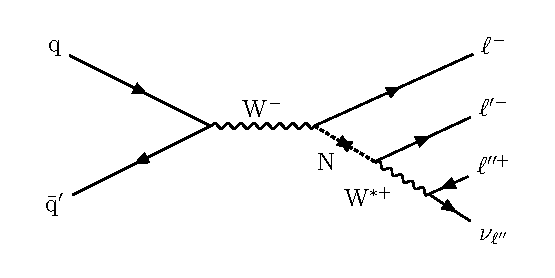
\includegraphics[width=0.48\textwidth]{Figures/c3/hnl_feyn.pdf}
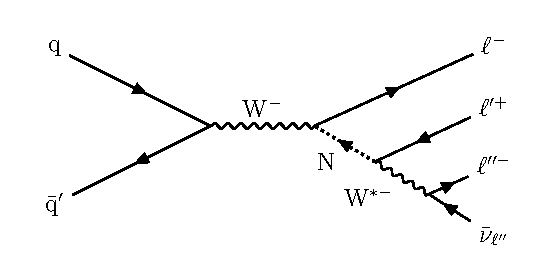
\includegraphics[width=0.48\textwidth]{Figures/c3/hnl_feyn_2.pdf}\\
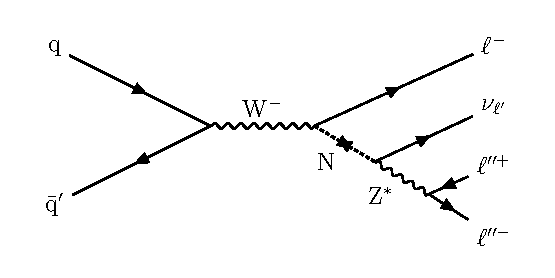
\includegraphics[width=0.48\textwidth]{Figures/c3/hnl_z_feyn.pdf}
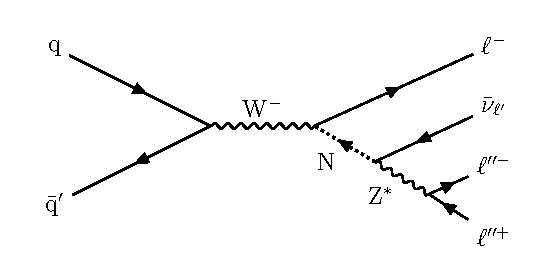
\includegraphics[width=0.48\textwidth]{Figures/c3/hnl_z_feyn_2.pdf}
\caption{Typical diagrams for the production of a HNL at the LHC 
($\hnl$) through its mixing with a SM neutrino, leading to a
final state with three charged leptons and a neutrino.
The HNL decay is mediated by either a $W$ (top row) or a $Z$ (bottom
row) boson.
In the diagrams on the left, $\hnl$ is assumed to be a Majorana
neutrino, thus $\ell$ and $\ell^\prime$ in the $W^\ast$-mediated
diagram (top) can have the same electric charge, with lepton-number
violation (LNV).
In the diagrams on the right instead, the $\hnl$ decay conserves the
lepton number (LNC) and can be either a Majorana or a Dirac
particle. Therefore $\ell$ and $\ell^\prime$ in the
$W^\ast$-mediated diagram (top right) have always opposite charge.
If \hnl couples exclusively to a single lepton-neutrino generation,
then $\ell$ and $\ell^\prime$ (or $\nu_{\ell^{\prime}}$) always belong
to the same lepton generation, and the lepton flavor is conserved
(LFC). If \hnl couples to multiple lepton families instead, then the
lepton flavor can be violated, $\ell\neq\ell^\prime$ (LFV).}
\label{fig:c3hnldiagram}
\end{figure}



\clearpage

\subsection{Previous and current results}
